\chapter{Tecnologías}
Una vez introducidos en el proyecto y con los objetivos marcados se hablara de las tecnologías usadas para el desarrollo de la aplicación. Las cuatro principales tecnologías en las que gira el proyecto son: Mongodb, Express, Angular2 y Node.
\begin{figure}[H]
    \centering
    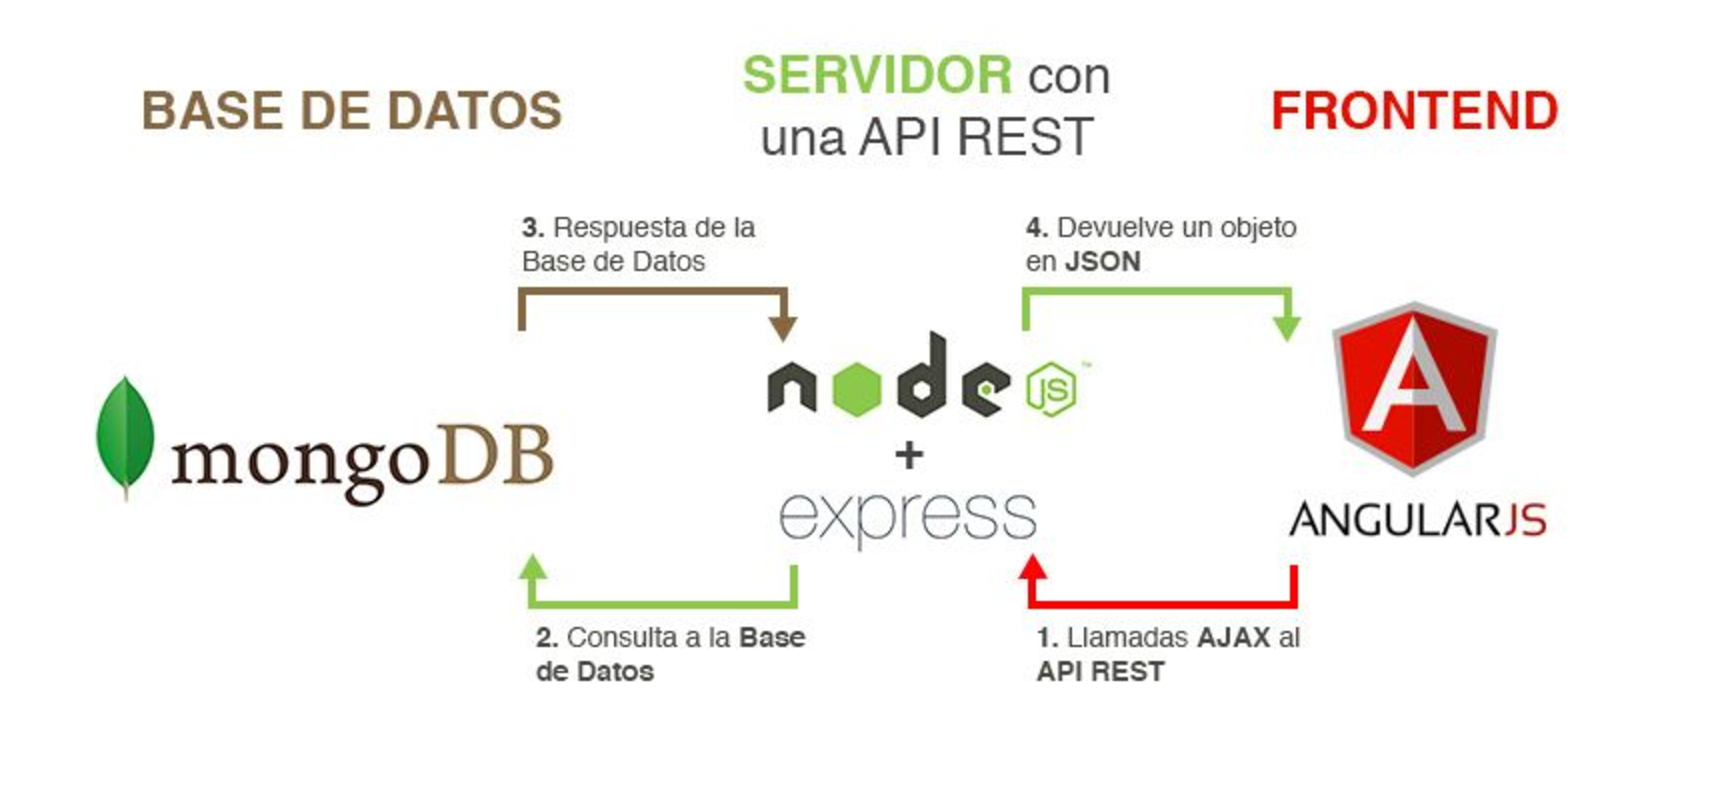
\includegraphics[width=140mm]{scheme.png}
    \caption{Esquema MEAN}
\end{figure}
En este esquema podemos ver como se comporta el stack MEAN, el cual hemos utilizado para el desarrollo de nuestra app. En este capítulo vamos a explicar como se comporta este paquete de 4 tecnologias: 


\section{MongoDB}
\begin{figure}[H]
    \centering
    
\includegraphics[width=40mm]{mongo.png}
\end{figure}
\subsection{Introduccion}

Mongo es una base de datos no relacional (NoSQL) de código abierto que guarda los datos en documentos tipo JSON (JavaScript Object Notation) pero en forma binaria (BSON) para hacer la integración de una manera más rápida. Se pueden ejecutar operaciones en JavaScript en su consola en lugar de consultas SQL. Además tiene una gran integración con Node.js con los driver propio y con Mongoose. Debido a su flexibilidad es muy escalable y ayuda al desarrollo ágil de proyectos web.

MongoDB esta orientado para servicios que necesiten una persistencia basada en documentos, al contrario que otros sistemas de base de datos noSQL como Cassandra, el cual esta orientado para logs, o como Redis que necesita una persistencia basada en colas de mensajes.

Estamos ante la era de lo que Martin Fowler llama “Polyglot
persistence”. Hay que decidir el tipo de persistencia a
utilizar para despues usar el tipo de persistencia que mas
se amolde a nuestras necesidades.

Las caracteristica que hacen tan importante a esta base de datos son las siguientes:



\begin{itemize}

    \item Está orientada a documentos. Lo que quiere decir que en un único documento es capaz de almacenar toda la información necesaria que define un producto, un cliente, etc, aceptando todo tipo de datos sin tener que seguir un esquema predefinido.
    
    \item Da respuesta a la necesidad de almacenamiento de todo tipo de datos: estructurados, semi estructurados y no estructurados. 
    
    \item Tiene un gran rendimiento en cuanto a escalabilidad y procesado de la información.
    
    \item Da respuesta a la necesidad de almacenamiento de todo tipo de datos: estructurados, semi estructurados y no estructurados. 
    
    \item Puede procesar la gran cantidad de información que se genera hoy en día..
    
    \item Permite a las empresas ser más ágiles y crecer más rápidamente, creando asi nuevos tipos de aplicaciones.
    
    
\end{itemize}

\subsection{MongoDB}

MongoDB esta escrito en C++, su version de 32 bits solo puede alcanzar 2GB, por este motivo la version de 32 bits no es recomendable usarla en produccion.
\begin{lstlisting}[language=JSON] 
{
    name: "mario",
    age: 24,
    preferences: [
        "programming",
        "nosql",
        "javascript"
    ]
}

\end{lstlisting}


Esto es un documento en Mongo, los cuales se almacenan en colecciones y estas a su vez en bases de datos. Estas colecciones poseen un esquema flexible y totalmente dinamico lo que hace que la velocidad de computo sea muy alta. Las bases de datos no se crean manualmente, primero se define la base de datos a usar y luego se inserta un documento en alguna coleccion.

\begin{lstlisting}[language=JSON] 
    > show dbs
    > use pruebanosql
    > show colections
    > db.users.insert({"name":"mario", "age":24})
\end{lstlisting}

Un problema que tiene Mongo, es que no soporta transacciones de multiples documentos, sin embargo puede proporciona operaciones atómicas en un solo documento. A menudo, estas operaciones atómicas de nivel de documento son suficientes para resolver los problemas que requerían transacciones en una base de datos relacional. Por ejemplo en Mongo se pueden incrustar datos relacionados en matrices anidadas o documentos anidados dentro de un solo documento y actualizar todo el documento en una sola operación atómica. Por este motivo los servicios que requieren de transacciones como los bancos o entidades economicas, no utilizan Mongo debido a que es sensible a Hacker, debido a que no es capaz de hacer una sola operación atomica en dos documentos.

Otro posible problema podria ser la excesiva cantidad de memoria RAM que puede consumir MongoDB, aunque es posible ejecutar mongo en una maquina con una pequeña cantidad de memoria RAM libre. Pero si es cierto que Mongo usa automaticamente toda la memoria libre del equipo como su cache, es por esto por lo que los monitores de recursos muestran que mongo utiliza una gran cantidad de memotria, pero su uso es dinámico. Es decir que si otro proceso de repente necesita mayor espacio de memoria RAM, MongoDB liberara parte de su memoria asignada para el otro proceso.

\subsection{Fragmentación (Sharding)}
\begin{figure}[H]
    \centering
    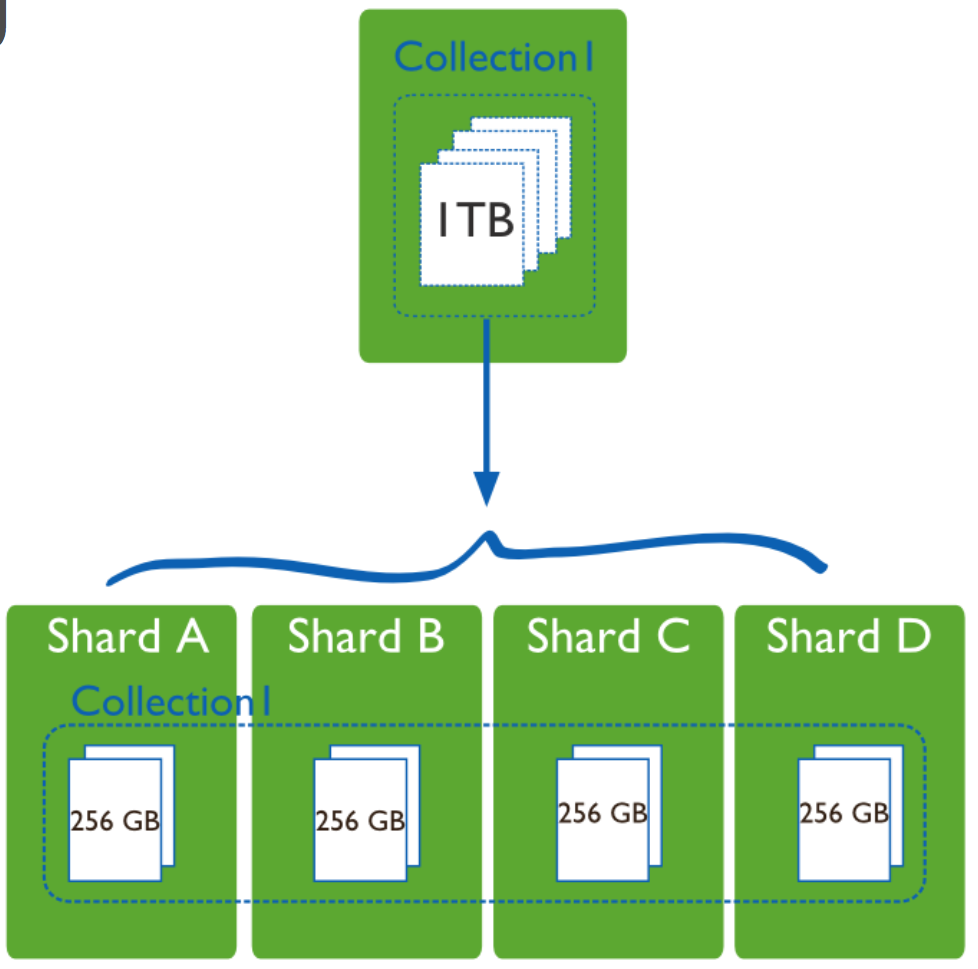
\includegraphics[width=90mm]{shard.png}
    \caption{Sharding}
\end{figure}
¿Que es el Sharding? Cuando el proyecto que estas llevando a cabo empieza a tener un numero de peticiones de acceso elevado , empiezas a notar que tu base de datos va mas lento de lo normal. Para este problema tienes dos soluciones, una actualizar toda la insfraestruztura para soportar la demanda o empezar a utilizar el sharding.

El sharding, es el modo en el que hacemos nuestra base de datos escalable. En lugar de tener una coleccion en una base de datos, la tendriamos en varias bases de datos distribuidas, de modo que a la hora de consultar los datos de dicha coleccion, los recuperaremos como si de una unica base de datos se tratase. Todo esto de encontrar la base de datos lo hace Mongo de forma transparente. Cuando hacemos consultas, tenemos un enrutador llamado "MongoS", el cual mantendra un pequeño pull de conexiones a los distintos host.

Los fragmentos estarán formados por replica set, de modo que
si creamos tres fragmentos, cada uno de los cuales tiene una
replica set con tres servidores, estaríamos hablando de un
total de nueve servidores. Para saber en que fragmento debe
consultar para recuperar datos de una coleccion ordenada, se
utilizan rangos y shard key, de modo que se torcea la colecicion en rangos y se les asigna un id a cada rango, de este modo que cuando se consulte la coleccion debemos proporcionar el shardKey.




\section{Express}

\begin{figure}[H]
    \centering
    
\includegraphics[width=90mm]{express.png}
\end{figure}

\subsection{Introduccion}
Express es un framework por encima de Node.js que permite crear servidores web y recibir peticiones HTTP de una manera sencilla, lo que permite también crear APIs REST de forma rápida.

Express es una plataforma ligera para construir aplicaciones web usando NodeJS. Nos ayuda a organizar las aplicaciones web en el lado del servidor. En la web de ExpressJS, lo describen como "un framework de desarrollo de aplicaciones web minimalista y flexible para Node.js". Sin duda el exito de express radica en lo sencillo que es usarlo, y además abarca un sin número de aspectos que muchos desconocen pero son necesarios.

De entre las tantas cosas que tiene este framework podemos destacar:

\begin{itemize}

\item \textbf{Router}
\item \textbf{Manejo de peticiones}
\item \textbf{Configuracion de la aplicacion}
\item \textbf{Middleware}
\end{itemize}

Para comenzar, y suponiendo que tienes ya instalado node y npm, lo único que es necesario hacer es lo siguiente:

\begin{lstlisting}[language=JSON] 
    > npm install -g express
\end{lstlisting}

Una vez instalado express puedes utilizar express NOMBRE-DEL-APP lo cual te creara una estructura personalizada y los archivos necesarios para comenzar a trabajar con el mismo. Haz cd NOMBRE-DEL-APP npm install para instalar automaticamente las dependencias.

\subsection{Server.js}

En una aplicación escrita con express existe una estructura interna bien definida y es como sigue:


\begin{itemize}

    \item \textbf{Modúlos o archivos externos} Importamos todos los módulos o archivos externos que nuestra app vaya a necesitar. El bloque, o mejor dicho la línea, que viene a continuación es la más importante de todas, ya que se encarga de instanciar Express y asignarlo a la variable app, la cual se utilizará a partir de ahora para configurar los parámetros de Express.
    
    \begin{lstlisting}[language=JSON] 
    var app = express();
   \end{lstlisting}
   
   El siguiente bloque sirve para configurar e iniciar algunos componentes de Express. Destacar la línea, app.use(express.static(...)), en la cual se configuran los objetos estáticos (imágenes, hojas de estilo, etc.) que debe servir Express, los cuales se encuentran en la carpeta public. Esta configuración permite también que los elementos estáticos puedan ser accedidos como si se encontrasen en el directorio raíz del proyecto, de forma que para acceder a las imágenes ubicadas en /public/images se haría con la URL http://localhost:3000/images.
    \begin{lstlisting}[language=JSON] 
    app.use(bodyParser.json());
    app.use(bodyParser.urlencoded({ extended: false }));
    app.use(cookieParser());
    app.use(express.static(path.join(__dirname, 'public')));
   \end{lstlisting}
   
    
    \item \textbf{Conectamos a la base de datos} La segunda parte de nuesta app express, es conectarnos a la base datos. 
    
    \item \textbf{Importamos controladores y modelos de la base de datos} Una vez conectados a la base de datos importamos los controladores y los modelos de nuestra base de datos.
    
    
   \item \textbf{Rutas} Las rutas son definitivamente la parte más importante de tu aplicación, porque si estas no están definidas, no existiria una interfaz para él cliente.
   
   Como podemos ver una ruta esta especificada de la siguiente forma:
   \begin{lstlisting}[language=JSON] 
    app.VERBO(PATH, ACCION)
   \end{lstlisting}
   
   VERBO: Puede ser: GET, POST, PUT, DELETE y así para cada uno de los verbos HTTP. 
   
   PATH: Define la dirección de acceso.
   
   ACCION: Que es lo que se tiene que hacer.
   
   \item \textbf{Listen} Por último es importante que tu aplicación este disponible en algún puerto.
   \begin{lstlisting}[language=JSON] 
    app.listen(3000);
   \end{lstlisting}
   
\end{itemize}

Express esconde muchas funcionalidades internas de Node, lo que te permite sumergirte en el código de tu aplicación y conseguir tus objetivos de forma muy rápida. Es fácil de aprender y te deja cierta flexibilidad con su estructura.
Por algo es el framework más popular de Node. Algunos nombres destacados que usan Express son:

\begin{itemize}

\item \textbf{MySpace}
\item \textbf{LinkedIn}
\item \textbf{Segment.io}
\end{itemize}



\section{Angular 2}

\begin{figure}[H]
    \centering
    
\includegraphics[width=80mm]{a2.jpg}
\end{figure}


\subsection{Introduccion}

Angular 2 es un framework JS para la parte cliente o Frontend de una aplicación web, que respeta el paradigma MVC y permite crear Single-Page Applications (Aplicaciones web que no necesitan recargar la página), de manera más o menos sencilla. Es un proyecto mantenido por Google y que actualmente está muy en auge.

Para crear apps en Angular 2 necesitamos:

\begin{itemize}

\item \textbf{Componemos plantillas HTML (templates) con el markup de Angular 2}
\item \textbf{Escribimos Componentes para gestionar esas plantillas}
\item \textbf{Encapsulamos la lógica de la aplicación en Servicios}
\item \textbf{Entregamos el componente raíz de la app al sistema de arranque de Angular 2 (bootstrap).}
\end{itemize}

Veamos como se relacionan estos elementos en el diagrama de arquitectura típico, sacado de la web de Angular 2:

\begin{figure}[H]
    \centering
    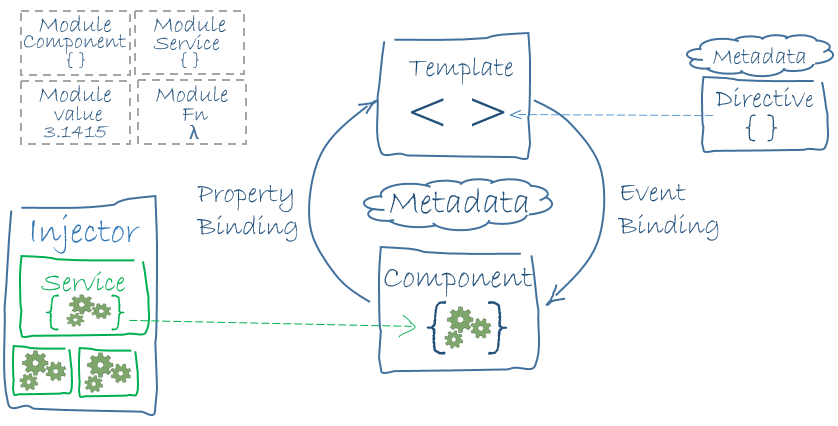
\includegraphics[width=110mm]{angular2Architecture.png}
\end{figure}

Podemos identificar los 8 bloques principales de una app con Angular 2:
\begin{itemize}

\item \textbf{Modulo} Igual que con su predecesor, las apps de Angular 2 son modulares. Un módulo, típicamente es un conjunto de código dedicado a cumplir un único objetivo. El módulo exporta algo representativo de ese código, típicamente una única cosa como una clase. Los modulos se pueden exportar e importar:

 \begin{lstlisting}[language=JSON] 
//app/app.component.js
    export class AppComponent {
        //aqui va la definicion del componente
    }
 
//app/main.js
    import { AppComponent } from './app.component';
\end{lstlisting}
   
Hay módulos que son librerías de conjuntos de módulos. Las librerías principales de Angular 2 son:
\begin{itemize}
\item \textbf{@angular/core}
\item \textbf{@angular/common}
\item \textbf{@angular/router}
\item \textbf{@angular/http}
\end{itemize}

\item \textbf{Componente} Un Component controla una zona de espacio de la pantalla que podríamos denominar vista. El componente define propiedades y métodos que están disponibles en su template, pero eso no te da licencia para meter ahí todo lo que te parezca. Haciendo un símil con AngularJS (Angular 1), un componente vendría a ser un controlador que siempre va ligado a una vista.
\item \textbf{Template} El Template (cuyo concepto ya existía en Angular 1), es lo que nos permite definir la vista de un Componente.
Igual que su predecesor, el template de Angular 2 es HTML, pero decorado con otros componentes y algunas directivas: expresiones de Angular que enriquecen el comportamiento del template.

Como vemos, además de elementos HTML normales como<h2> y <div>, hay otros elementos desconocidos en nuestro lenguaje de markup:
\begin{itemize}
\item \textbf{*ngForg}
\item \textbf{todo.subject}
\item \textbf{(click)}
\item \textbf{[todo]}
\item \textbf{todo-detail}
\end{itemize}

\item \textbf{Metadatos}
\item \textbf{Data Binding} Uno de los principales valores de Angular es que nos abstrae de la lógica pull/push asociada a insertar y actualizar valores en el HTML y convertir las respuestas de usuario (inputs, clicks, etc) en acciones concretas. Escribir toda esa lógica a mano (lo que típicamente se hacía con JQuery) es tedioso y propenso a errores, y Angular 2 lo resuelve por nosotros gracias al Data Binding.
\begin{itemize}
\item \textbf{Interpolación} Hacia el DOM.
{{todo.subject}}
\item \textbf{Property binding} Hacia el DOM. 
[todo]="selectedTodo"
\item \textbf{Event binding} Desde el DOM. (click)="selectTodo(todo)"

\item \textbf{Two-way binding} (Desde/Hacia el DOM) input [(ngModel)]="todo.subject"
\end{itemize}
\item \textbf{Directiva}
\item \textbf{Servicio}
\item \textbf{Dependency Injection}  Una dependencia en tu código se produce cuando un objeto depende de otro. Hay diferentes grados de dependencia, pero tenerla en exceso hace que testear tu código sea complicado o que algunos procesos se ejecuten más tiempo de la cuenta.
La inyección de dependencias es un método por el cual damos a un objeto las dependencias que requiere para su funcionamiento. 
\end{itemize}

Angular permite extender el vocabulario de tu HTML con directivas y atributos para crear componentes dinámicos. Si alguna vez has hecho una página web dinámica sin Angular te habrás dado cuenta de ciertas complicaciones frecuentes, como el data binding, validación de formulario, manejador de eventos con DOM (Document Object Model) y otras muchas. Angular presenta una solución “todo-en-uno” a esos problemas.
La curva de aprendizaje para Angular es muy pequeña, lo que explica que mucha gente se este pasando a este framework. La sintaxis es simple y sus principios básicos como el data binding (vinculación de elementos de nuestro documento HTML con nuestro modelo de datos) y la inyección de dependencias son sencillas de entender.


\section{Node}

\begin{figure}[H]
    \centering
    
\includegraphics[width=80mm]{node.png}

\end{figure}
Node es un entorno de programación en JavaScript para el Backend basado en el motor V8 de JavaScript del navegador Google Chrome y orientado a eventos, no bloqueante, lo que lo hace muy rápido a la hora de crear servidores web y emplear tiempo real. Fue creado en 2009 y aunque aún es joven, las últimas versiones lo hacen más robusto además de la gran comunidad de desarrolladores que posee.

\begin{itemize}
\item \textbf{NPM}.Uno de los beneficios de Node es su gestor de paquetes, npm (node package manager) y nos permite gestionar todas las dependencias y módulos de una aplicación. Al igual que Ruby tiene RubyGems y PHP tiene Composer, Node tiene npm.
Viene ya incluido con Node y permite que nos bajemos una serie de packages/paquetes para satisfacer nuestras necesidades. Los packages amplían la funcionalidad de Node y este sistema de paquetes una de las cosas que hace a Node tan potente.
La capacidad de tener una serie de códigos que puedes reutilizar en todos tus proyectos es increíble y hace que el desarrollo sea mucho más sencillo. Puedes combinar varios paquetes para crear aplicaciones complejas.
\end{itemize}
